\documentclass{../source/zjureport}

\major{信息工程}
\name{周灿松}
\title{实验设计报告}
\stuid{3190105055}
\college{信息与电子工程学院}
\date{\today}
\lab{东4-216}
\course{电子电路设计实验二}
\instructor{李锡华、施红军、叶险峰}
\grades{}
\expname{实验设计报告}
\exptype{设计实验}
\partner{宋凯}

\begin{document}
    \makecover
    \makeheader

    \section{实验目的}
        \begin{enumerate}
            \item 学习掌握用Arduino UNO 设计倒计时定时器;
            \item 学习掌握PCB 电路板的设计和制作;
            \item 学习掌握Arduino UNO 扩展板的设计与制作;
            \item 学习掌握旋转编码器的使用。
        \end{enumerate}
    
    \section{实验任务与要求}
        \begin{enumerate}
            \item 用Arduino UNO 设计倒计时定时器,要求如下:设定倒计时时间若干(设定标准时间数
            组),通过旋转编码器选择,时间到时报警。
            \item 设计电路,完成相应器件的选择,制作Arduino UNO 扩展板。
            \item 编制与调试倒计时定时器程序。
            \item 将制作的扩展板与Arduino UNO 板组装后,进行系统联调。
        \end{enumerate}

    \section{实验原理}
        \subsection{Arduino UNO板}
        Arduino UNO R3具有14个数字输入/输出引脚,6个模拟输入/输出。在本次倒计时电路设计中,我们以
        Arduino UNO R3作为整体电路的控制器,通过不同引脚在不同情况下输出不同电压控制七段数码管以及
        蜂鸣器,以此实现倒计时功能

        \subsection{七段数码管}
            \subsubsection{数码管构成}
            7 段数码管一般由8 个发光二极管组成,其中由7 个细长的发光二极管组成数字显示,另外一个圆形
            的发光二极管显示小数点。


            当发光二极管导通时,相应的一个点或一个笔画发光。控制相应的二极管导通,就显示出各种字符,尽
            管显示的字符形状有些失真,能显示的字符数量也有限,但其控制简单,使有也方便。发光二极管的阳
            极连在一起的称为共阳极数码管,阴极连在一起的称为共阴极数码管。
            \newpage
            \begin{figure}[thp]
                \centering
                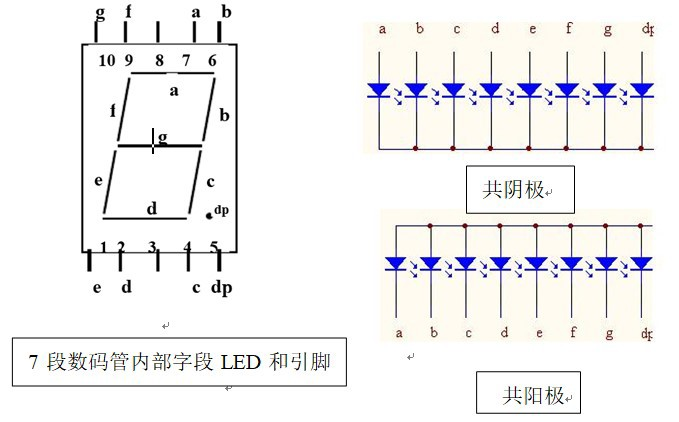
\includegraphics{figures/七段数码管结构.jpg}
                \caption{七段数码管结构}
            \end{figure}

            \subsubsection{驱动方式}
            七段数码管具有静态驱动和动态驱动两种方式。


            静态驱动方式中每一个发光二极管均有一个输出引脚控制,采用此种驱动方式编程实现更加简单,数码
            管亮度也更高,缺点则是它需要的管脚较多,由于arduino的输出管脚数目有限,我们不采用此种驱动
            方式,而是选用动态驱动。


            动态驱动则是利用了发光二极管的余辉效应以及人的视觉暂存现象。在此种驱动方式中,我们将所有数码管的同名端连在一起,在同一时刻,施加在所有数码管上的控制信号均相同,但同一时刻只有一个数码管处于导通状态。通过控制COM端,我们令所有数码管轮流点亮,	当扫描速度足够快时,看上去就像所有数码管同步显示了一样。

        \subsection{蜂鸣器}
        蜂鸣器按是否有驱动分为有源蜂鸣器和无源蜂鸣器两种。此处的“源”指的是震荡源而非电源,有源蜂鸣器只需要我们施加一个电压给他就可以响,无源蜂鸣器则需要用一个特定频率的方波对他进行驱动。为了设计简单,此次实验我们选用了有源的蜂鸣器。

        \subsection{旋转编码器}
         旋转编码器是一种数字器件,它有着两个输出A和B,当旋转时,输出A、B会有变化,通过变化的不同我们可以判断出旋转编码器是顺时针旋转还是逆时针旋转,如此便可利用旋转编码器控制倒计时的时间

    \newpage
    \section{电路及程序设计}
        \subsection{总体电路图}
        \begin{figure}[thp]
            \centering
            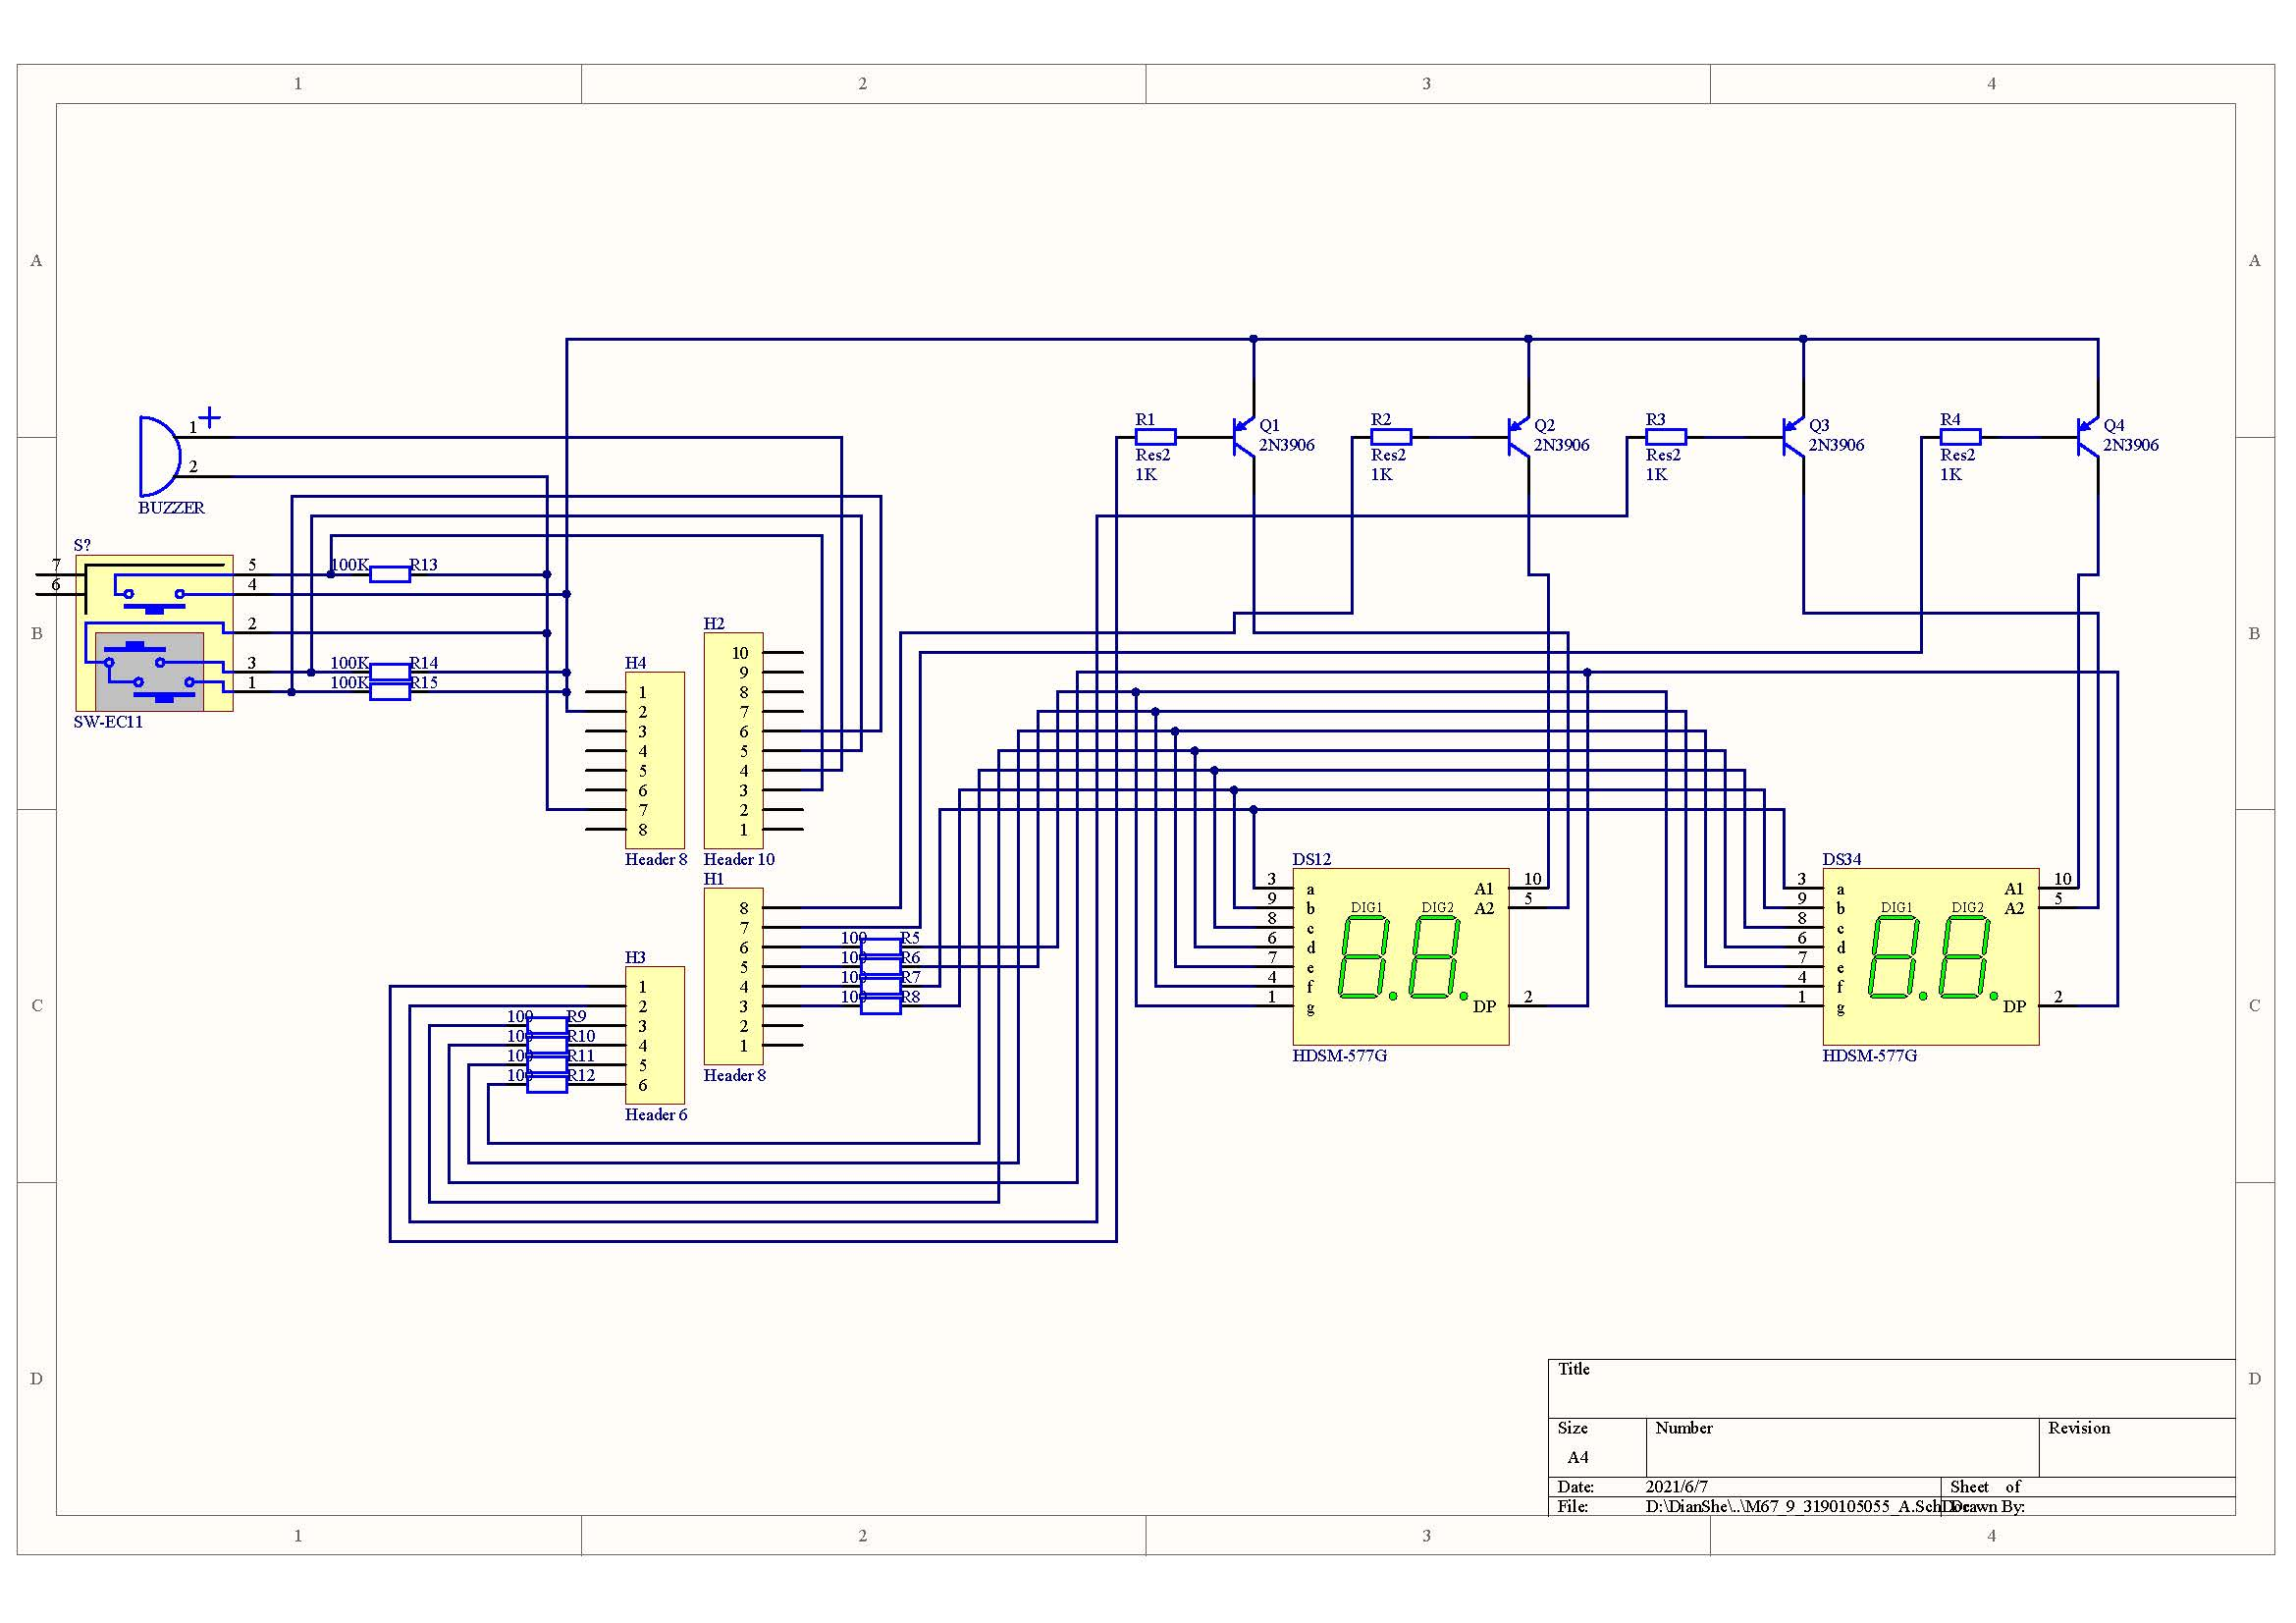
\includegraphics[scale = 0.55]{figures/Schematic Prints.jpg}
            \caption{原理图}
        \end{figure}

        \subsection{时间显示模块}
        在本次实验中我们选用了两个两位的七段数码管作为剩余时间显示,DS12显示分钟,DS34显示剩余秒数。


        在线路连接上,我们将两个数码管的1-4,6-9号引脚一一对应连接后接到Arduino的输出管脚上,如此便可将显示信号同时输出到四个七段数码管上。而控制数码管导通与否的5、10号引脚,我们分别将其接入四个三极管上,此处三极管作为开关管使用,通过控制三极管轮流导通即可实现四个七段数码管的轮流点亮。同时,在线路与arduino连接前,我们先接入了一个电阻作为保护电阻,防止出现问题。

        \subsection{旋转编码器模块}
        EC11型旋转编码器有五个引脚,其中1、3脚为信号A、B,4、5脚为开关,2脚接地。


        在转动旋转编码器时,会产生如下波形,通过观察A、B信号变化的过程便可判断出是顺时针还是逆时针旋转。
        \newpage
        \begin{figure}[thp]
            \centering
            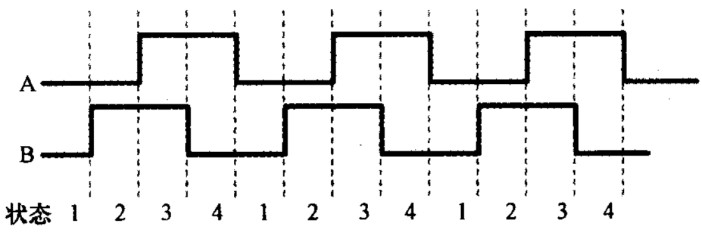
\includegraphics{figures/旋转编码器波形.jpg}
            \caption{旋转编码器波形}
        \end{figure}
        \textbf{代码设计:}
        \begin{lstlisting}[name=旋转编码器部分代码,
            language = c
            ]
            //右旋返回为1,左旋为-1,不旋为0
            int getEncoderTurn()
            {
                // return -1,0,or +1 
                static int oldA=LOW; 
                static int oldB=LOW; 
                int result = 0;
                int newA = digitalRead(aPin);
                int newB = digitalRead(bPin);
                if (newA != oldA || newB != oldB)
                {
                    // something has changed
                    //当信号B从低电平变化到高电平时,如果A为低电平,则说明状态是从左到右变化,反之则反
                if(oldB == LOW && newB == HIGH){
                    result = oldA*2 - 1;
                    }
                }
                oldA = newA;
                oldB = newB;
                return result;
            }
        \end{lstlisting}


        \subsection{蜂鸣器模块}
        因为我们采用了有源蜂鸣器,所以只需要将蜂鸣器加在一个输出引脚上,控制该引脚的输出电压,即可控制蜂鸣器的启动与否。

    \section{主要仪器设备}
    Arduino UNO R3,EC11型旋转编码器,两个两位七段数码管,四个三极管,电阻若干

    \section{PCB版图绘制}
        \subsection{绘制步骤}
        \begin{enumerate}
            \item 绘制原理图并编译
            \item 创建PCB文件,并将原理图同步至PCB图中
            \item 放置各个元件,此步需要注意引脚位置的放置,不然后续可能无法与Arduino板连接
            \item 选择层级为信号层,隐藏无关元素进行手动布线
        \end{enumerate}
        
        \subsection{PCB图}
            \begin{figure}[htp]
                \centering
                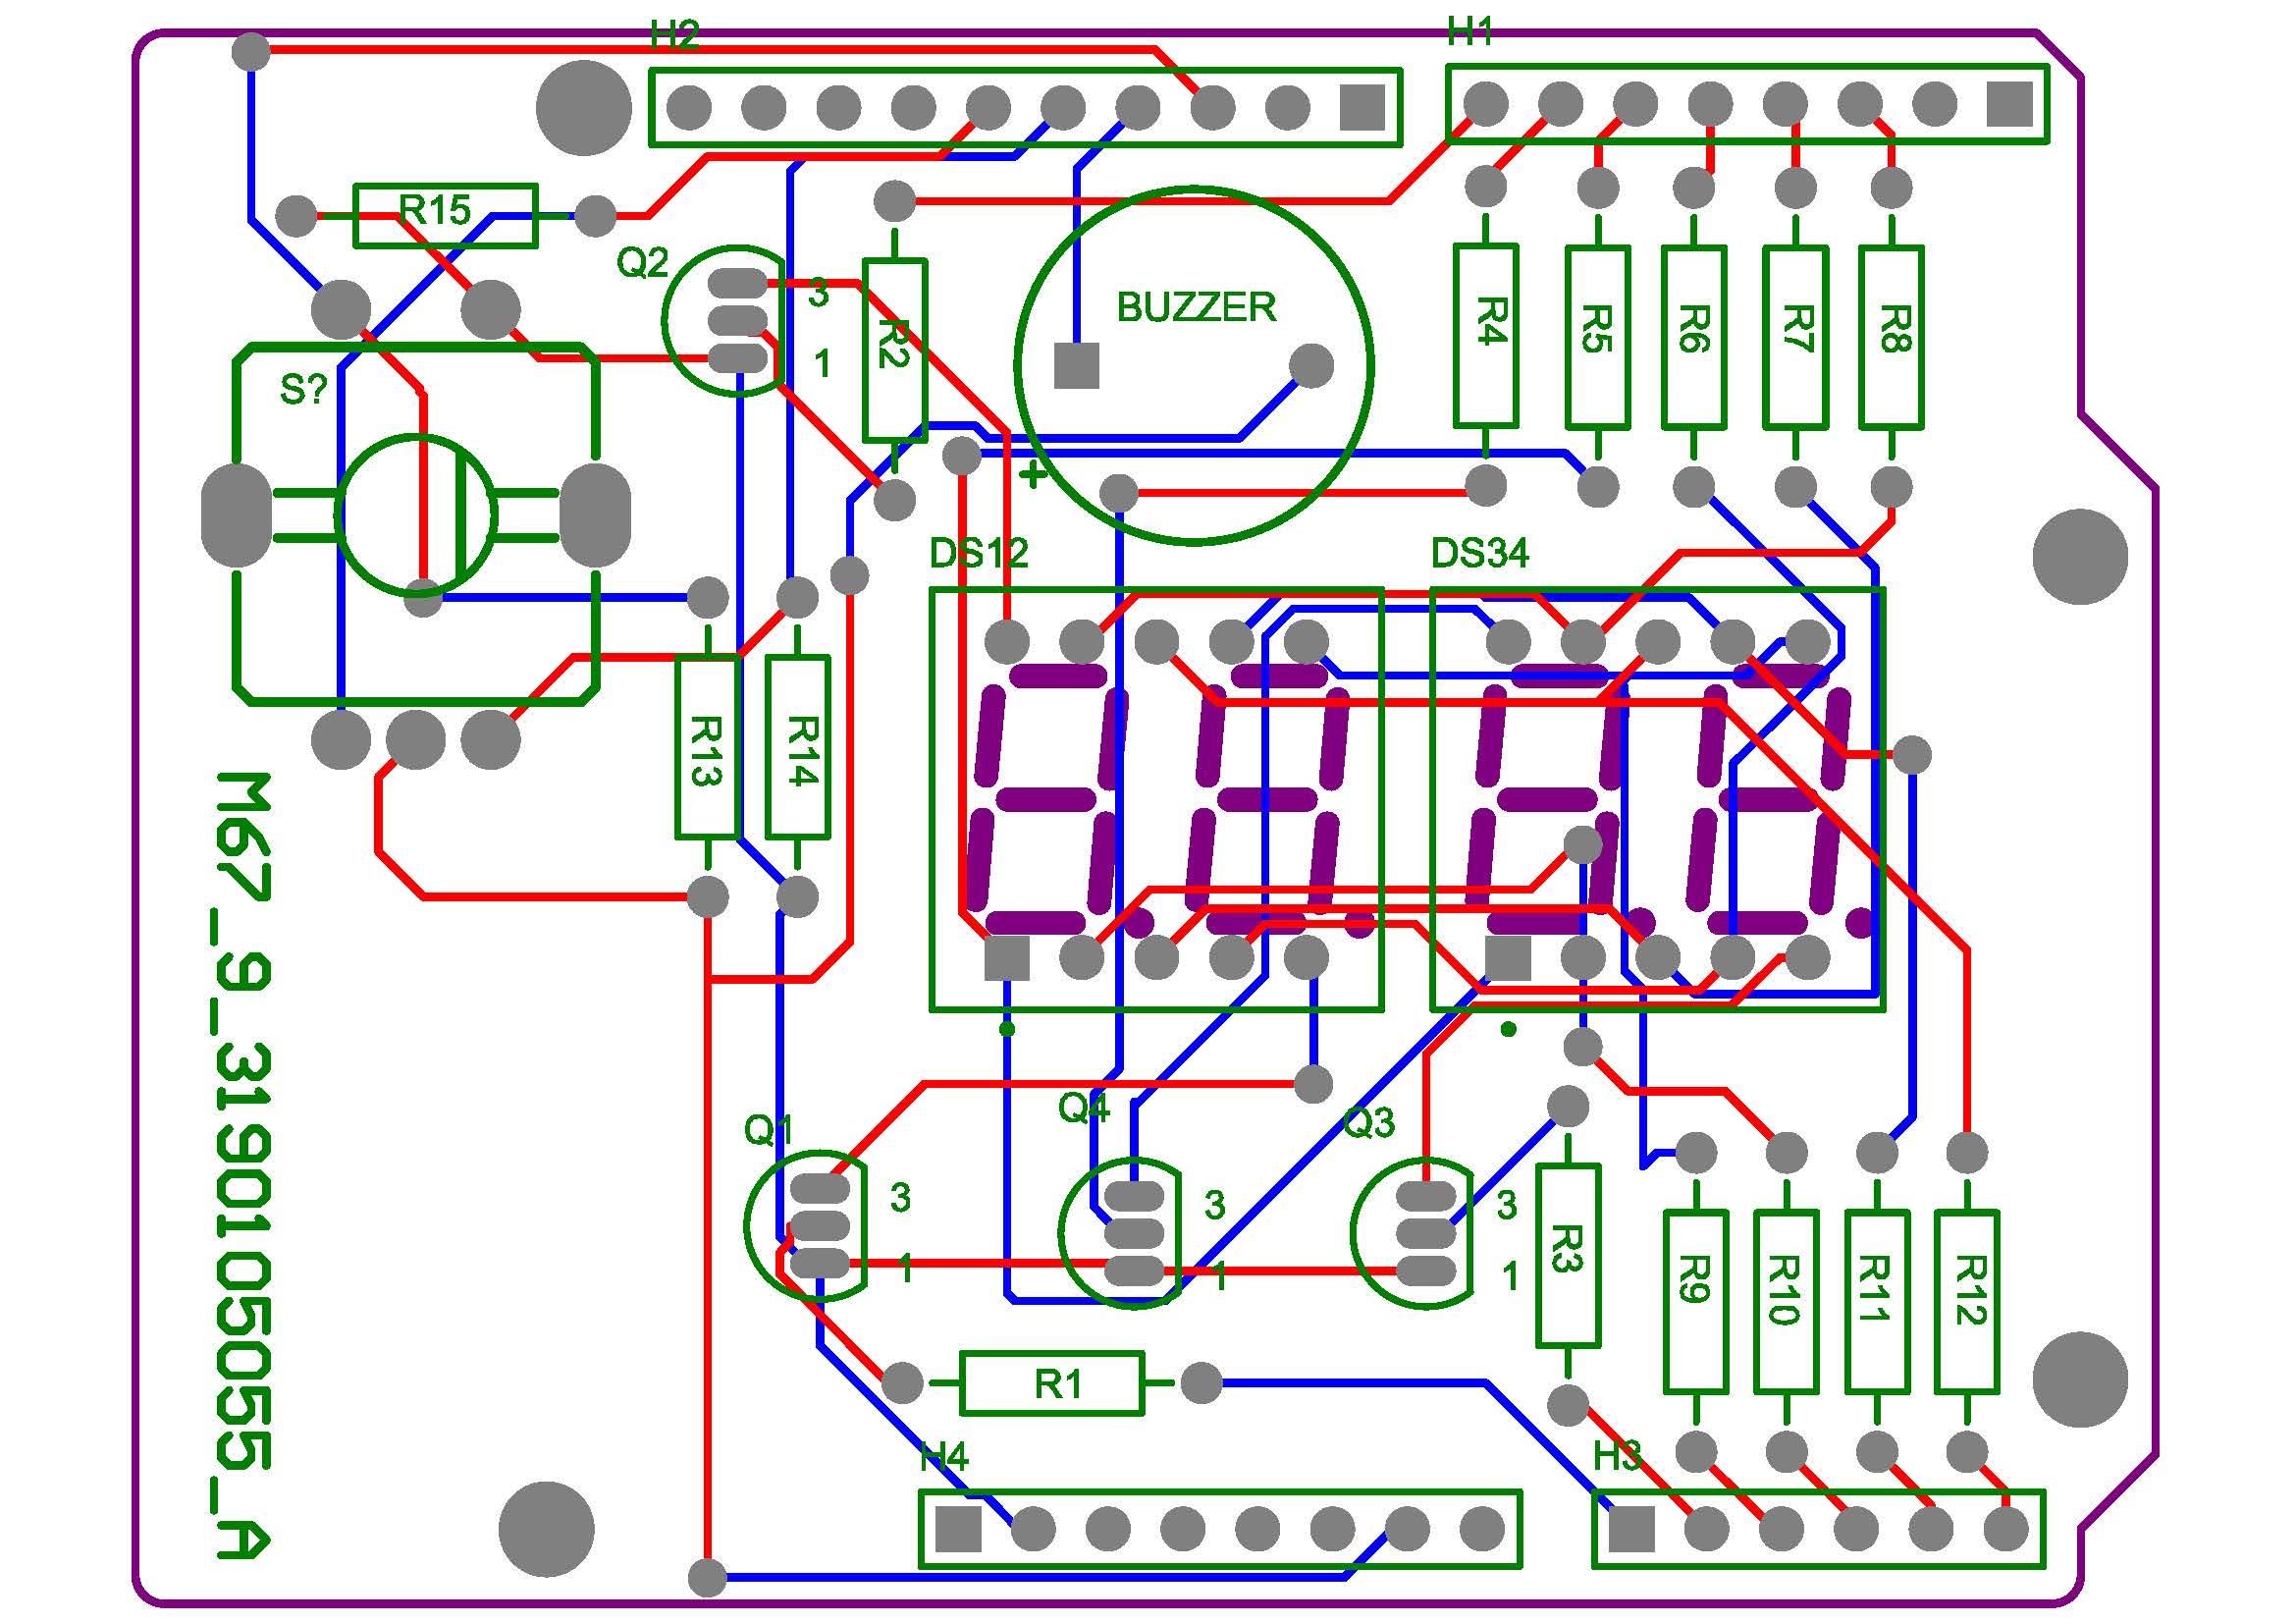
\includegraphics[scale = 0.55]{figures/PCB2.jpg}
                \caption{PCB板图}
            \end{figure}

    \section{调试}
        \subsection{焊接}
        按照电路设计选取元件,按高度从低到高的原则将其焊接到PCB板上。
        \newpage
        \begin{figure}[htp]
            \centering
            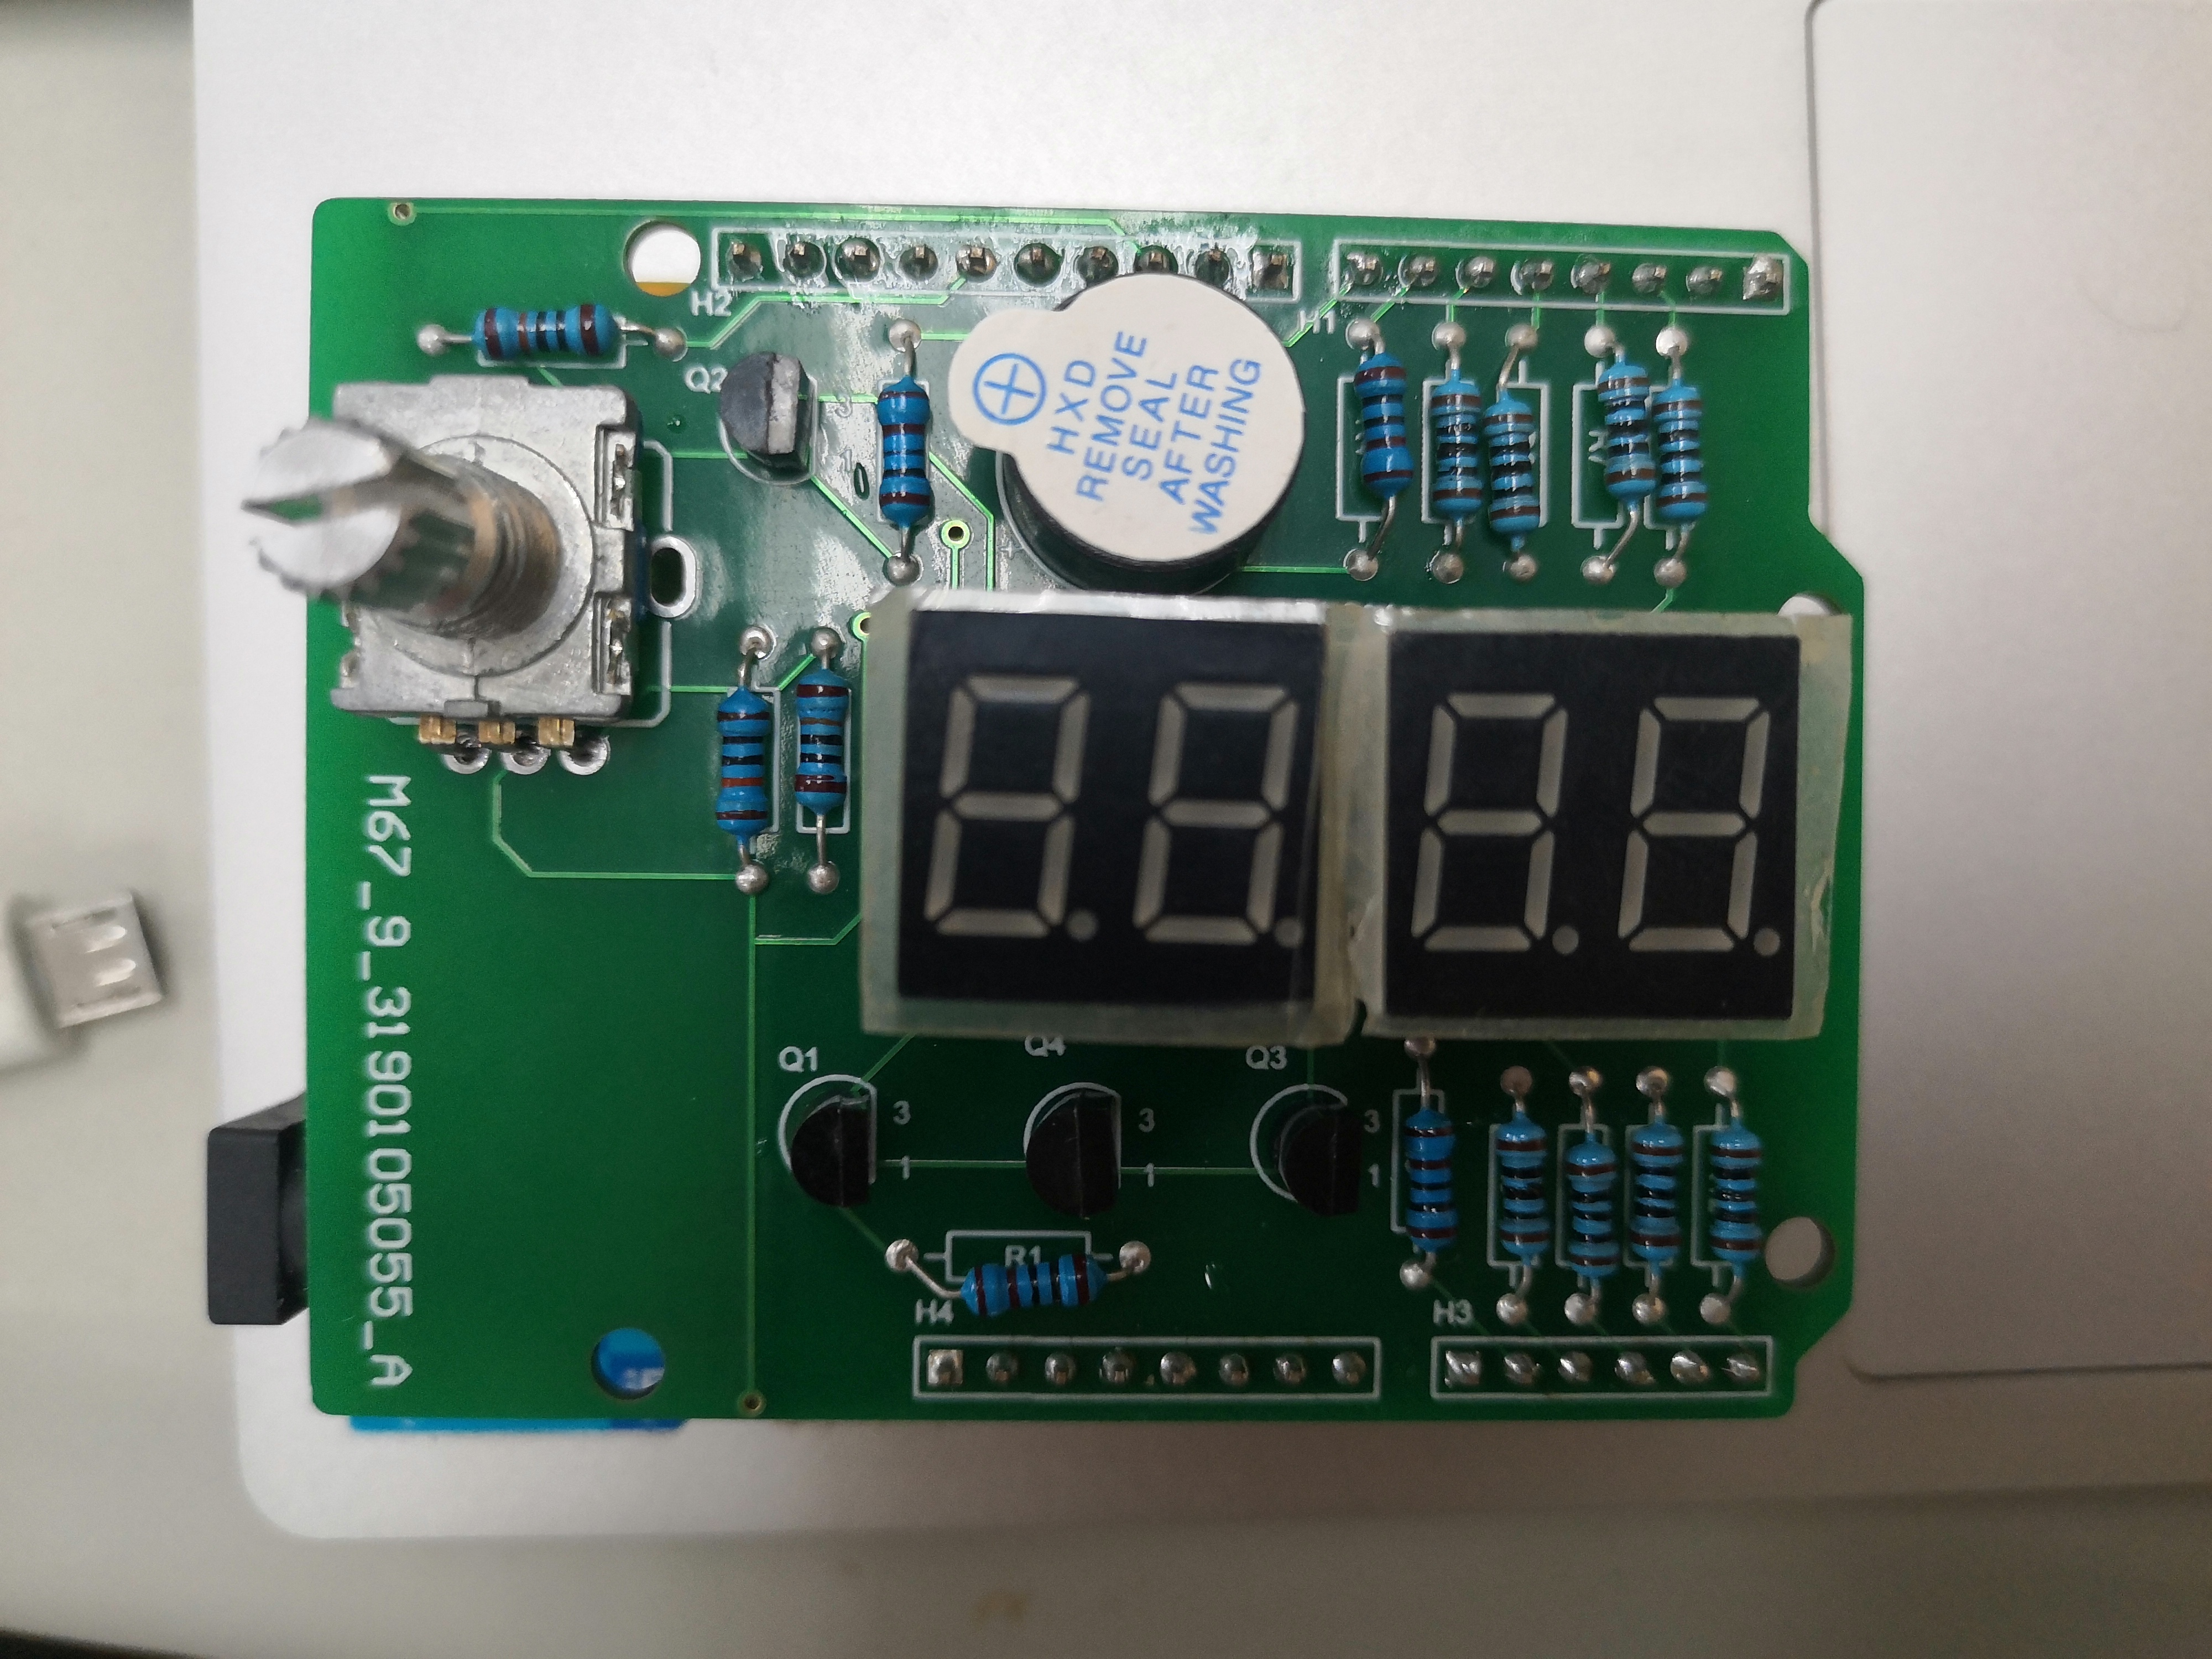
\includegraphics[scale = 0.09]{figures/焊接结果.jpg}
            \caption{焊接成果}
        \end{figure}

        \subsection{调试}
        1.将代码拷入Arduino之中,数码显示如下:
        \begin{figure}[!htp]
            \centering
            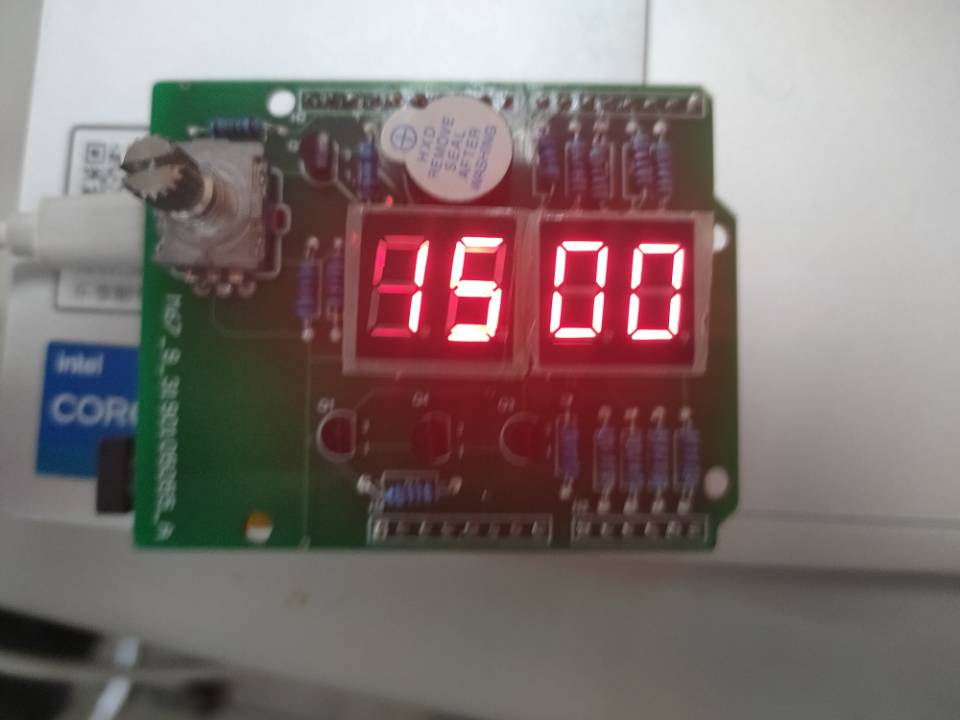
\includegraphics[scale = 0.28]{figures/数码显示.jpg}
            \caption{能正常显示数字}
        \end{figure}


        2.按以下步骤测试功能:
        \begin{enumerate}
            \item 按下旋转编码器,测试是否能正常倒计时以及到时间能否报警
            \item 拧动旋转编码器,测试能否正确改变设定时间
            \item 设定一时间,将Arduino断电,然后上电测试其能否记住上次设定时间
        \end{enumerate}

        
        功能均正常,不足之处见下文

        \subsection{调试中的问题及解决方案}
            \subsubsection{问题}
            七段数码管出现闪烁,时间切换不够流畅

            \subsubsection{解决方案}
            修改代码中以下部分,修改方案见\textbf{注释}
            \begin{lstlisting}[name=数码管闪烁解决方案]
        void process()
            {
                //将此循环中的循环次数由100调小,寻找合适次数,大概在50左右比较合适
                for (int i = 0; i < 100; i++) 
                {
                    int change = getEncoderTurn();
                    if (stopped)
                    {
                         changeSetTime(change);
                    }
                    else
                    {
                        updateCountingTime();
                    }
                }
                if (timerMinute == 0 && timerSecond == 0)
                {
                    digitalWrite(buzzerPin, HIGH);
                }
            }
            \end{lstlisting}


    \section{思考题}
        \textbf{1.将图4.15 中的数码管换成共阴的,分别说明电路和程序要做怎样的修改}
            
        
        电路图可以不做修改,保持原有线路不变。


        程序需要改动两个地方:第一处将$byte\  digits[10][8]$中的1和0互换;二则是将setDigit函数中digitalWrite第二个参数中的不等号换为等号。


        \textbf{2.考虑倒计时定时器的应用,例如如何控制定时加热,简要介绍实现的电路。}
            

        和控制蜂鸣器时间结束后长鸣原理类似。另寻一个数字输出口,将其与电阻丝一端相连,另一端接地,时间结束后,数字输出口持续输出高电平即可。


        \textbf{3.如何通过修改程序,消除秒钟滴答声。}


        删除updateCountingTime函数中以下代码,或者移除delay(10):
        \newpage
        \begin{lstlisting}[name=待删除代码]
            digitalWrite(buzzerPin, HIGH);
            delay(10);
            digitalWrite(buzzerPin, LOW);
        \end{lstlisting}


    \section{讨论总结、体会}
    在前期电路设计过程中,其实也遇到了不少的问题,因为以前没有设计过Arduino拓展板,所以在最开始拿到题目的时候陷入了迷茫之中,不知道从何而起。在反复读了参考资料之后,才渐渐有了眉目。因为老师的资料中给了电路图,我们设计电路的时候困难较少,但是当进入面包板调试过程后,我们发现事情并不像自己想象中的那么顺利,出现了以下几个问题:


    首先,七段数码管和A4那个pdf中的数码管封装不同。拿到器件之后,我们不知道怎么去接线,但通过互联网查找到了该型号数码管的器件手册(后面发现老师给了器件手册截图),事情变得顺利起来了。
    

    其次,旋转编码器给我留下了深刻的印象,因为不懂旋转编码器的工作原理,我们就照猫画虎地按照图上接线,最后在测试功能的时候发现拧动编码器无法改变计时的多少。在课后,我将板子连到自己电脑进行串口调试后发现拧动编码器并不会令A,B信号改变,所以我大胆推测是线路接错了。在网上学习了旋转编码器的工作原理之后,我发现自己将1,3号脚直接接地了,这也就导致了A,B信号输入始终为低电平。将其改接高电平之后,成功地解决了问题。
    

    在设计电路并进行面包板调试时,因为电子电路设计实验二是开放实验,因为以前没有做过类似的实验,出现了各种各样的问题。但是在解决问题的过程中,我也很明显地感受到了自己的成长。实践是最能够检验自己所学的途径,在实践的过程中,每解决一个问题都能够获得一股巨大的成就感,这种成就感也能激励着我继续学习下去。同时,在实践中才能够更加透彻地理解各个器件地使用方法,就如数码管的驱动方式,不进行实验始终觉得动态驱动很虚无飘渺,但实验后才会发现这的确能够正确地运行。


    调试过程中,除了焊接三极管时需要注意不要将三个电极焊在一起了,焊接总体而言问题不大。在调试过程中,数码管出现了闪烁的情况,极其影响观感,在研究了代码之后,发现是process函数中的循环次数过大,但是也不能改的过小,改得太小也会导致数码显示管出现模糊的情况,最终在反复尝试之后将循环次数确定在了50次,使得模糊和闪烁之间取得了一个平衡。
    
    
    在这次的实验设计工作中,我学到的更多的是电路设计的方法,跟着老师给的大致方案,一步一步地将一个能够实现具体功能的电路构建好,并在面包板上实现。虽然其中设计的部分偏少,更多地是跟着老师的方案把东西做出来,但是这个过程也让我管中窥豹,知道了电路设计的大致流程,也在一定程度上培养了对于电路设计的兴趣,以及自己的动手能力。其次,在这个过程中也学会了AD软件的基本操作,懂得了利用AD软件绘制PCB版图的过程。

    \newpage
    \lstinputlisting[caption = 完整代码]{code/project.ino}

\end{document}